\section{Sch1 Class Reference}
\label{classSch1}\index{Sch1@{Sch1}}
Inheritance diagram for Sch1::\begin{figure}[H]
\begin{center}
\leavevmode
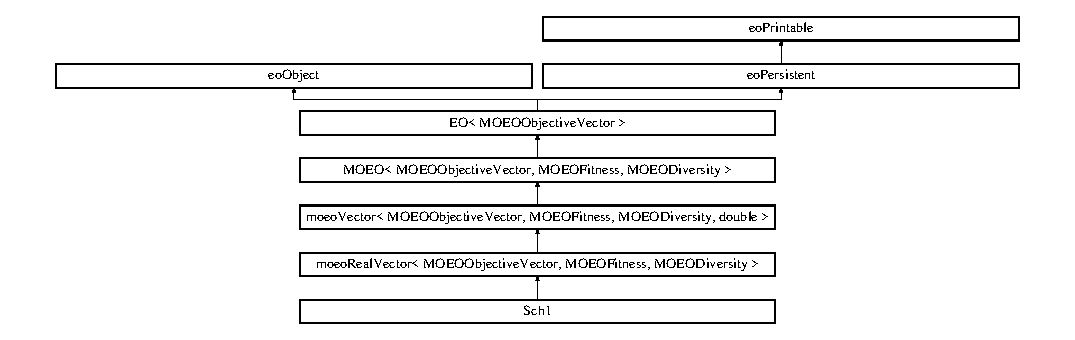
\includegraphics[height=4.11765cm]{classSch1}
\end{center}
\end{figure}
\subsection*{Public Member Functions}
\begin{CompactItemize}
\item 
\bf{Sch1} ()\label{classSch1_3ddc72f40539bfe0d5bb8d977b6655c0}

\end{CompactItemize}


\subsection{Detailed Description}




Definition at line 44 of file Sch1.cpp.

The documentation for this class was generated from the following file:\begin{CompactItemize}
\item 
Sch1.cpp\end{CompactItemize}
